
% Stashing things up here for later

%\begin{quote}
%Quote goes here
%\end{quote}



\documentclass[12pt]{article}

% Packages
\usepackage{setspace} % for adjusting line spacing
\usepackage{parskip} % for controlling paragraph spacing
\usepackage{fontspec} % for setting fonts
\usepackage{fancyhdr} % for custom headers and footers
\usepackage{biblatex} % for bibliography management
\usepackage[margin=1in]{geometry} % for setting margins
\usepackage{titlesec} % for customizing section headings
\usepackage{etoolbox} % for adjusting environment parameters
\usepackage{graphicx} % for including graphics
\usepackage{dot2texi}
\usepackage{tikz}
\usepackage{caption} % for customizing captions
%\usepackage{sectsty} % for modifying section headings

% Line spacing
\setstretch{2}

% Paragraph spacing
\setlength{\parskip}{0pt}

% Define indentation length
\newlength{\myindent}
\setlength{\myindent}{3em}

% Set global text alignment to ragged-right
\raggedright

% Paragraph indentation
\setlength{\parindent}{\myindent}

% Font
\setmainfont{Times New Roman}

% Page style
\pagestyle{fancy}
\fancyhf{} % clear all header and footer fields
\fancyhead[R]{\thepage} % page number on the right side
\fancyhead[L]{\small CONSTRUCTION UNIONS: HISTORICAL-COMPARATIVE}
\renewcommand{\headrulewidth}{0pt} % remove header rule

% Disable hyphenation
%\pretolerance=10000
%\tolerance=2000 
%\emergencystretch=10pt
%\hyphenpenalty=10000
%\exhyphenpenalty=10000

% Bibliography setup
% \addbibresource{My Library.bib}
% \ExecuteBibliographyOptions{sorting=none} % unsorted bibliography

% Define custom section headings
%\titleformat{\section}[block]{\MakeUppercase\normalfont\fontsize{12}{14}\selectfont}{\thesection.}{0.5em}{}
\titleformat{\section}[block]{\normalfont\fontsize{12}{14}\selectfont}{\thesection.}{0.5em}{}
\titleformat{\subsection}[block]{\itshape}{\thesubsection.}{0.5em}{}
\titleformat{\subsubsection}[runin]{\normalfont\itshape}{\hspace{\myindent}\thesubsubsection.}{0.5em}{}[.]

% Redefine the quote environment
\renewenvironment{quote}
  {\list{}{\leftmargin=\parindent\rightmargin=0pt}%
   \item\relax}
  {\endlist}

\renewenvironment{abstract}
  {\par\noindent\centering\textbf{Abstract}\par\noindent\raggedright}
  {\par}

% Redefine the quote environment to make it single-spaced
\renewenvironment{quote}
  {\begin{singlespace}\list{}{\leftmargin=\parindent\rightmargin=0pt}%
   \item\relax}
  {\endlist\end{singlespace}}

\begin{document}

\begin{titlepage}
  \thispagestyle{fancy}
  \fancyhead[L]{Running head: CONSTRUCTION UNIONS: HISTORICAL-COMPARATIVE}
  \centering
  \vspace*{1.95in}
  {\LARGE Construction Union Agreements:\par Union Organizing in Historical-Comparative Perspective\par}
  \vspace{1.2in}
  {Matthew A. Carson\par}
  \vspace{0in}
  {University of California, Los Angeles\par}
  \vspace{0.5in}
  {\today\par}
\end{titlepage}

% Set page numbering to roman for preliminary pages
\pagenumbering{roman}

% Add abstract page
\begin{abstract}
US Building Trade unions organize their workers differently. Most labor unions compel employers to negotiate, but the Building Trades engage in voluntary negotiations, relying on workers' skill levels rather than strike leverage. This approach correlates with their frequent political deviations from the broader US labor movement, particularly in opposing progressive environmental policies and aligning more closely with the petrochemical industry on environmental issues, and not supporting single-payer healthcare. One view is that unions pursue their members’ interests narrowly, sacrificing broader working-class interests if they feel it is necessary to secure work for their members, and some suggest that the conservative stance of the Building Trades stems from their craft union tradition, in which workers are organized by craft and skill instead of by industry. However, using historical-comparative methods, I show that these arguments do not hold. Petrochemical unions have supported progressive policies, and other craft-based unions have endorsed single-payer healthcare. However, unlike the Building Trades, those unions have never used voluntary agreements. Consequently, they have experienced more conflicts with employers. These findings challenge traditional views and suggest that the Building Trades' conservative negotiation strategies significantly shape their political and policy positions, reinforcing an employer-union dynamic that limits challenging management.
\end{abstract}
\newpage

% Add table of contents
\tableofcontents
\newpage

% Set page numbering to arabic for main content
\pagenumbering{arabic}

\section{INTRODUCTION} \

Construction is one of the largest unionized sectors in the United States. In spite of this, labor research has largely not focused on construction unions (or what are often referred to as the Building Trades) but has largely focused on the ways in which workers in other industries organize. In some sense this is understandable. One of the largest periods of union growth in the US was in the 1930s, a period in which multiple violent strikes occurred, sometimes lasting for a month or longer. These events contributed to the rise of the Congress of Industrial Unionism (CIO), which was a federation of trade unions committed to industrial unionism, rather than craft unionism. Congress and President Franklin D. Roosevelt responded to these violent battles by enacting the Wager Act, which guaranteed the right for workers to organize and provided a framework for workers to petition for union representation in the workplace. This framework was largely adapted to the way that industrial unions were organizing at the time. Most unionization efforts, especially large-scale and prominent efforts, have used the industrial union model of organizing.

Construction unions in the US have a distinct approach to organizing their workers vis-a-vis other labor unions. While most labor unions typically compel employers to negotiate either through secret ballot elections or work stoppages, the Building Trades take a different route by engaging in voluntary negotiations. Their strategy hinges more on the skill levels of their workers than the leverage of strikes or official National Labor Relations Board elections, which use the state to compel the employer to negotiate. This unique approach often leads them to deviate politically from the broader US labor movement. Notably, they often oppose progressive environmental policies and tend to align more closely with the petrochemical industry on environmental issues. Additionally, they are not supportive of single-payer healthcare.

Some argue that this conservative stance of the Building Trades originates from their tradition of craft unionism, where workers are organized based on craft and skill rather than industry. However, historical-comparative analyses challenge this view. For instance, other unions with many members working in the petrochemical industry have backed progressive policies, including environmental policies, and other craft-based unions have endorsed single-payer healthcare despite organizing along craft lines instead of industry. The key distinction between these unions and their disparate political stances lies in the Building Trades' use of voluntary agreements, which minimizes conflicts with employers and constrains their ability to challenge management.

% Foner, Phillip S. History of the Labor Movement in the United States: Volume 2: From the Founding of the AFL to the Emergence of American Imperialism. New York: International Publishers, 1955; pp. 132–133.

\subsection{Craft Unionism vs. Industrial Unionism} \

Craft unionism is when workers are organized into a union by craft (occupation) rather than employer or industry. The earliest efforts in the US to organize workers collectively to assert the interests and preferences were generally organized around craft lines. Plumbers formed their union; machinists started one; so did the carpenters, and so on. Many of these early craft unions were successful, and eventually The American Federation of Labor (AFL) formed in 1886, bringing many of the labor unions at the time into a nationwide federation. Immediately many the constituent unions battled over craft jurisdiction. Who had the right to organize workers in the print room? Both the Machinists and the International Typographical Union claimed jurisdiction. As a result, one of the most important functions of the newly formed federation was to quell these jurisdictional fights.

Industrial unionism did not come until some time later. Industrial unionism is when workers are organized by employer or industry, regardless of their craft, occupation, or skill level. Many of the early craft unionists in the AFL were skeptical of indsutrial unionism. Many of the workers in mass production factories at the time were immigrants with no craft and little formal training. The craft union leaders in the AFL did not think that it would be possible to organize them because they did not have leverage that having a craft would equip the workers with. The jobs were largely repetitive and did not require a high-skill level. For example, standing in the same place and fastening the same bolts at the same place on a Model-T all day was not a craft in the way that being a machinist and working a lathe or being a pile driver and driving piles for a new bridge was.

\subsubsection{The Industrial Bargaining Approach}

The National Labor Relations Act (NLRA) sets forth the process that workers must follow to unionize a workplace. The National Labor Relations Board (NLRB) administers the NLRA. The NLRA specifies the processes that workers and union organizers should follow to form a union. The typical process begins with an effort to determine if there is a general interest in forming a union or joining a union among workers already hired. If there appears to be enough interest, “employee organizers typically collect union interest cards, petitions or other written statements from co-workers to show interest in union representation. Organizing efforts may be supported by an established union seeking to represent workers at a workplace. Workers may also form an independent union” (DOL n.d.:How can I form a union?). If enough cards are collected to demonstrate majority status, the workers may ask the employer to voluntarily recognize the union. If the employer refuses to voluntarily recognize the union, workers may strike and/or file a petition with the NLRB to request an election to certify the union and the collective bargaining representative of the workers (DOL n.d.; NLRB n.d.). Once the union has demonstrated that the majority of workers want union representation (either through voluntary recognition by the employer or through a NLRB election), the union and employer will attempt to reach an initial agreement. This type of agreement is called a Section 9(a) agreement.

\subsubsection{The Building Trades Approach}

In contrast to this approach, building and construction trade unions do not usually organize the workers at the workplace. They usually establish voluntary agreements with employers, which can be established before any employees are hired by the employer. Since these agreements can be established before any workers are hired, they are called prehire agreements, or in legalistic jargon, Section 8(f) agreements. Prehire agreements have a long history that predates their legitimation by Congress in 1959 with the passage of the Labor-Management Reporting and Disclosure Act (LMRA). In fact, prior to the LMRA, the NLRB had refused to take jurisdiction over the building and construction trades because their approach to union organizing was so different and in fact would be an unfair labor practice, a violation of the NLRA, if they were to take jurisdiction over the matter. So, whereas labor law is often discussed in terms of how the law constrains union organizing efforts, this is not the case with respect to prehire agreements used by the building and construction trades; they were already organizing this way prior to the passage of the LMRA.

This distinction between 9(a) and 8(f) agreements is useful because it underscores two very different orientations toward the boss and two very different approaches to mobilizing worker power. Perhaps most notable is the starting point of the unionization process. The former starts with the employees already hired. Sometimes it is primarily driven by union staff; other times, it can be driven more by shop floor organizers from the rank-and-file. Either way, the approach is to organize workers around issues they are facing in the workplace and compel the employer to negotiate a contract through coercive measures such as strikes or using the state as an instrument to compel the employer to bargain in good faith. The building and construction trade unions largely dispense with this approach, instead trying to entice employers on the basis of their members’ skill and training and by collaborating with the employers. (The building and construction trades are not forced by law to organize in this way; it is their choice whether to organize in this way or another way.)

\begin{figure}
  \centering
  \includegraphics[width=0.75\textwidth]{images/organizing_paths}
  \captionsetup{justification=centering, singlelinecheck=false, margin=2cm}
  \caption{The industrial mode of organizing (left), and the construction mode of organizing (right). Construction unions may follow either path, but other unions may not voluntarily negotiate the way that construction unions can.}
  \label{fig:organizing_paths}
\end{figure}

One practical reason for the development of prehire agreements in the building and construction trades is the temporary nature of the work. Because of the temporary nature of the work, many union halls maintain a hiring hall with dispatch procedures for members out of work. At the completion of the job assignment, laid off union members may return to the union’s hiring hall and make themselves available for employment somewhere else by signing the out of work list maintained by the union. The union will dispatch its members to jobs as needed by the employer. Because of this temporary nature of the job, organizing via the traditional route is much more challenging because workers are laid off so frequently and the employer has no permanent workforce, at least not in the way that other workplaces do. From that perspective, prehire agreements are a practical response to the specific unionization challenges faced in the construction industry. However, this particular arrangement has serious consequences for how construction unions must situate themselves in relation to the employer. That is to say, because of the voluntary nature of the agreements, the employer may simply choose to leave the collective bargaining relationship at the expiration of the contract. Thus, construction unions that follow this method of organizing generally must maintain a much more employer-friendly orientation than other unions who organize through the other route. Simply put, if the employer feels that the workers are pushing too hard in their enforcement of their contract or that the union has become too radical, the employer is free to leave at the next bargaining round.

Because of this threat, building trades unions have to be employer friendly. For example, the union does not have exclusive control over its training program. Instead, the Joint Apprenticeship Training Committee (JATC) oversees the training process and curriculum development. The JATC is a committee comprised of 50% labor and 50% management, each having equal share in controlling the apprenticeship program. 

\section{THE HIRING HALL}

The temporary nature of construction work gave rise to a different mode of organizing. Because of the temporary nature of construction work, construction unions (of the American Federation of Labor, AFL) organized a much different set of arrangements than the industrial unions (mostly in the Congress of Industrial Organizations, CIO) that came along later to organize around industry-wide lines. Rather than organize the workers on the shop floor to demand concessions and better working conditions from their employer, construction unions use their leverage as a particularly skilled workforce that employers needed to complete their projects. Because of this employer need for a particular skill set, the union workers could demand wages, working-conditions, fringe benefits, etc. In exchange for their labor. If employers are not willing to cede these demands, the skilled workers can withhold their labor, and employers will not be able to complete their projects. If employers are able to reach an agreement with the union, then a contract is crafted and a hiring hall established (or the employer is incorporated into an extant hiring hall). The hiring hall is a central component of the prehire contract arrangement. They go hand-in-hand. Its development is largely due to the particularly contingent nature of construction work:

\begin{quote}
	Many construction industry employers hire employees, as the need arises, to work on a particular project and to be laid off when their services are no longer required. Most construction workers are organized into union hiring halls. A hiring hall, or work referral system, is an arrangement under which a union that "has control of or access to a particular labor pool agrees to supply workers to an employer upon request." When an employer in the construction industry needs skilled workers for a project, he often seeks such workers from the union hiring hall. Historically, the practice in the construction industry was for the employer to sign an agreement with the hiring hall union which set the terms and conditions of employment for workers \textit{not yet hired}. These contracts, known as pre-hire agreements, often contemplated a tenure of years, spanning several projects. Rather than having to renegotiate the terms and conditions of employment on each new project, the employer was assured a ready supply of skilled workers and predictable labor costs upon which to base his bids on projects subcontracted by a general contractor. Furthermore, the construction worker had the benefit of a central clearinghouse for employment opportunities. (emphasis added; Murphy 1982 pp. 1014–1015)
\end{quote}

Construction unions had been operating in this way for many years prior to the exemption to majority status requirements that were carved out for construction unions in Section 8(f) as part of the Landrum-Griffin Labor-Management Reporting and Disclosure Act (LMRDA) of 1959. In fact, before its enactment, the prehire agreement constituted a violation of the law which had, up until that point, required the union to show that the majority of employees wanted representation from that particular union. Murphy (1982) explains how the particularities of the construction industry made other modes of union organizing and operation difficult:

\begin{quote}
	The periods of employment in the construction industry are often so short, however, that it is impracticable to complete the process of certifying a collective bargaining representative before a project ends and the employees are laid off. Furthermore, if an employer recognizes a union as bargaining representative of his employees, but the union is not in fact supported by a majority of his employees, the employer has committed the unfair labor practice of illegally assisting a union in violation of section 8(a)(1) of the National Labor Relations Act (NLRA). Pre-hire agreements, therefore, technically constituted illegal assistance of a union by the employer because agreements were signed prior to the union attaining majority status, indeed before the employer had even hired any employees. (pp. 1016-1017)
\end{quote}

To which the NLRB’s response was to ignore the violation until the 1959 passage of the LMRDA:

\begin{quote}
	The General Counsel for the Board recognized the need of the construction industry to have a skilled work force available for quick referral and adopted a policy of not issuing complaints against construction employers and unions entering into pre-hire agreements. Finally in 1959, Congress legitimized pre-hire agreements by enacting section 8(f) of the NLRA. (Murphy p. 1017)
\end{quote}

In Senate debate, many senators acknowledged that this way of organizing in the construction trades was long-standing and informally ignored by the Board and courts. For example, Senator Javits recognized that the Taft-Hartley law, which LMRDA was to amend, was not being applied at the time:

\begin{quote}
	We cannot apply the Taft-Hartley law to the building and construction field. We all know the law is not being applied in that field, and we might as well recognize the fact in the law. This is an essential amendment, and the sooner we adopt it the better. (“105 Congressional Record, 86th Congress, 1st Session (1959)”, p. 6395) 
\end{quote}

Nor was this a regulation "imposed from above" to stifle trade unionism the way that Taft-Hartley was a dozen years earlier. Senator Dirksen acknowledged that labor wanted this amendment and had even approached senators about it in the years before LMRDA’s passage:

\begin{quote}
	I remember that 2 years ago, when Mr. Richard Gray, the head of the Carpenters Union, came to the reception room with the General Counsel of the Department of Labor, they presented to us a proposal on the so-called prehiring agreements in the construction industry. They said, "This is what we want." (105 Congressional Record, 86th Congress, 1st Session (1959), p. 6414)
\end{quote}

A few years earlier in 1956, the United Brotherhood of Carpenters’ magazine, the Carpenter, the official publication of the union spoke favorably of the bill because it would allow contractors and building trades unions [to] carry on contractual relationships in the way they have for over 50 years" (https://archive.org/details/carpenter76unit/page/n5/mode/2up?view=theater pp. 7-8)

\begin{figure}
  \centering
  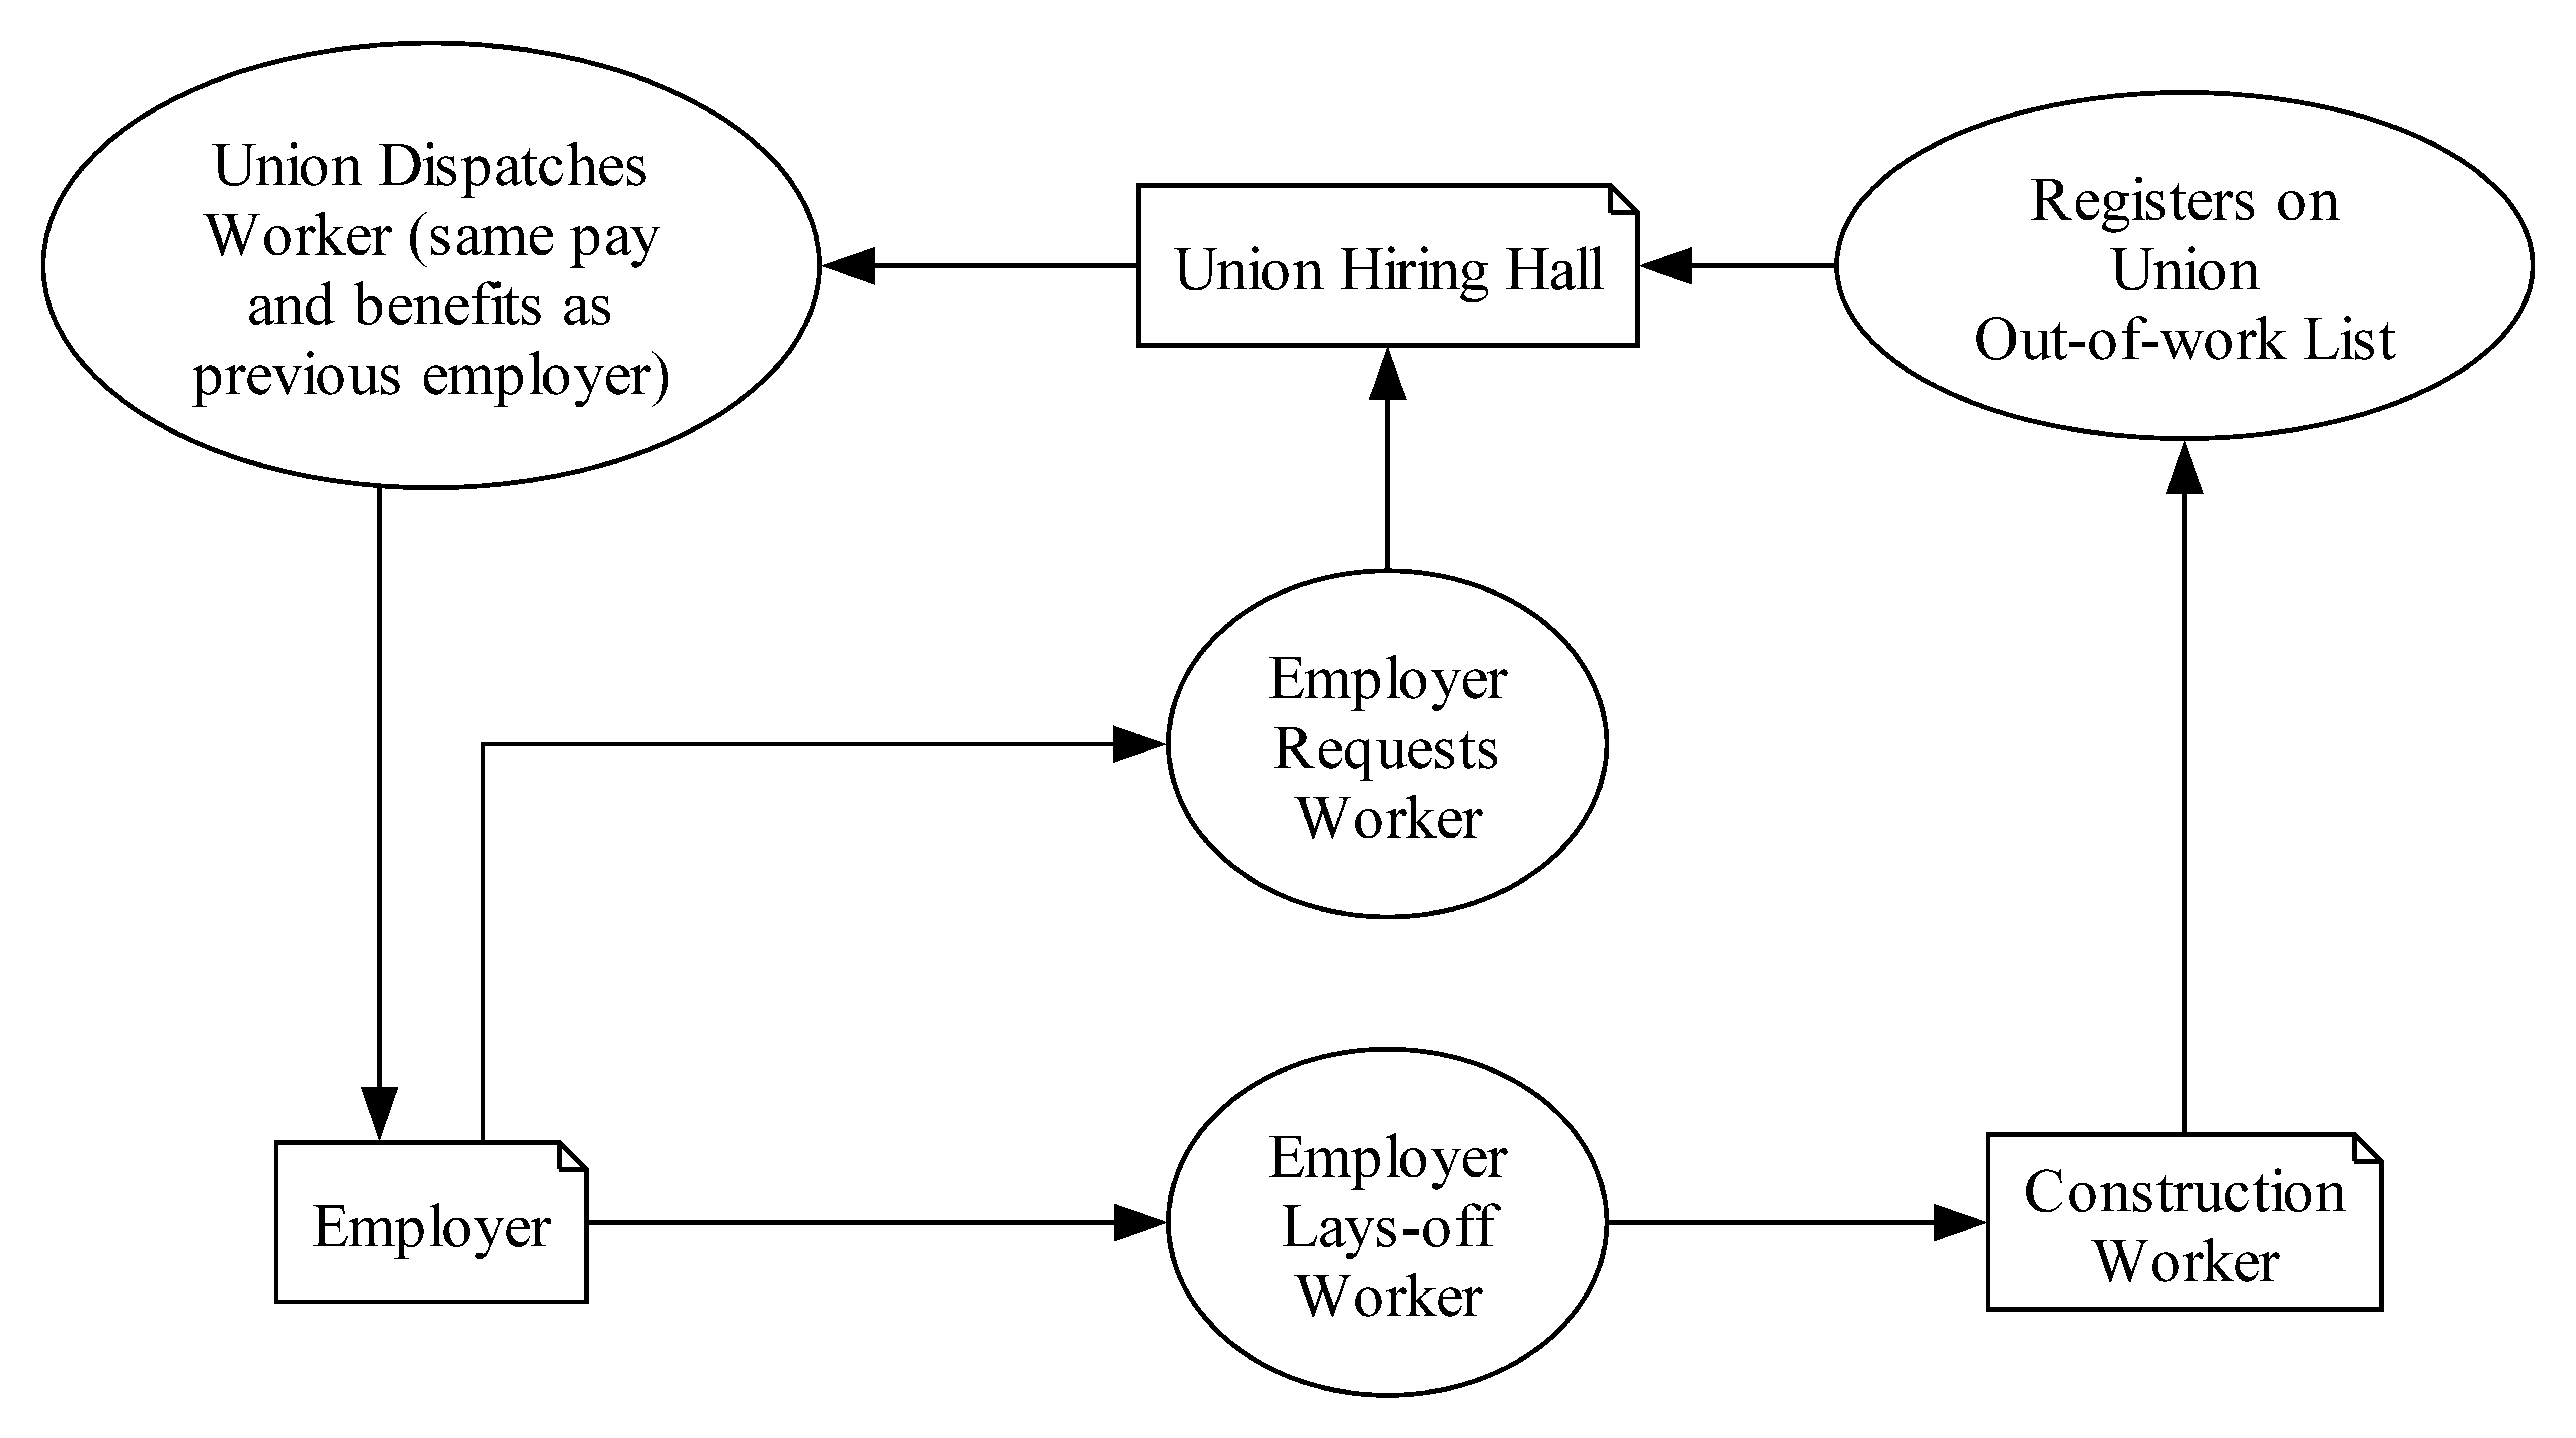
\includegraphics[width=0.8\textwidth]{images/hiring_hall}
  \captionsetup{justification=centering, singlelinecheck=false, margin=2cm} 
  \caption{Construction unions usually maintain a hiring hall. When employers require more workers for their projects, they contact the hiring hall to request workers to be dispatched to the job site.}
  \label{fig:hiring_hall}
\end{figure}

\begin{figure}
  \centering
  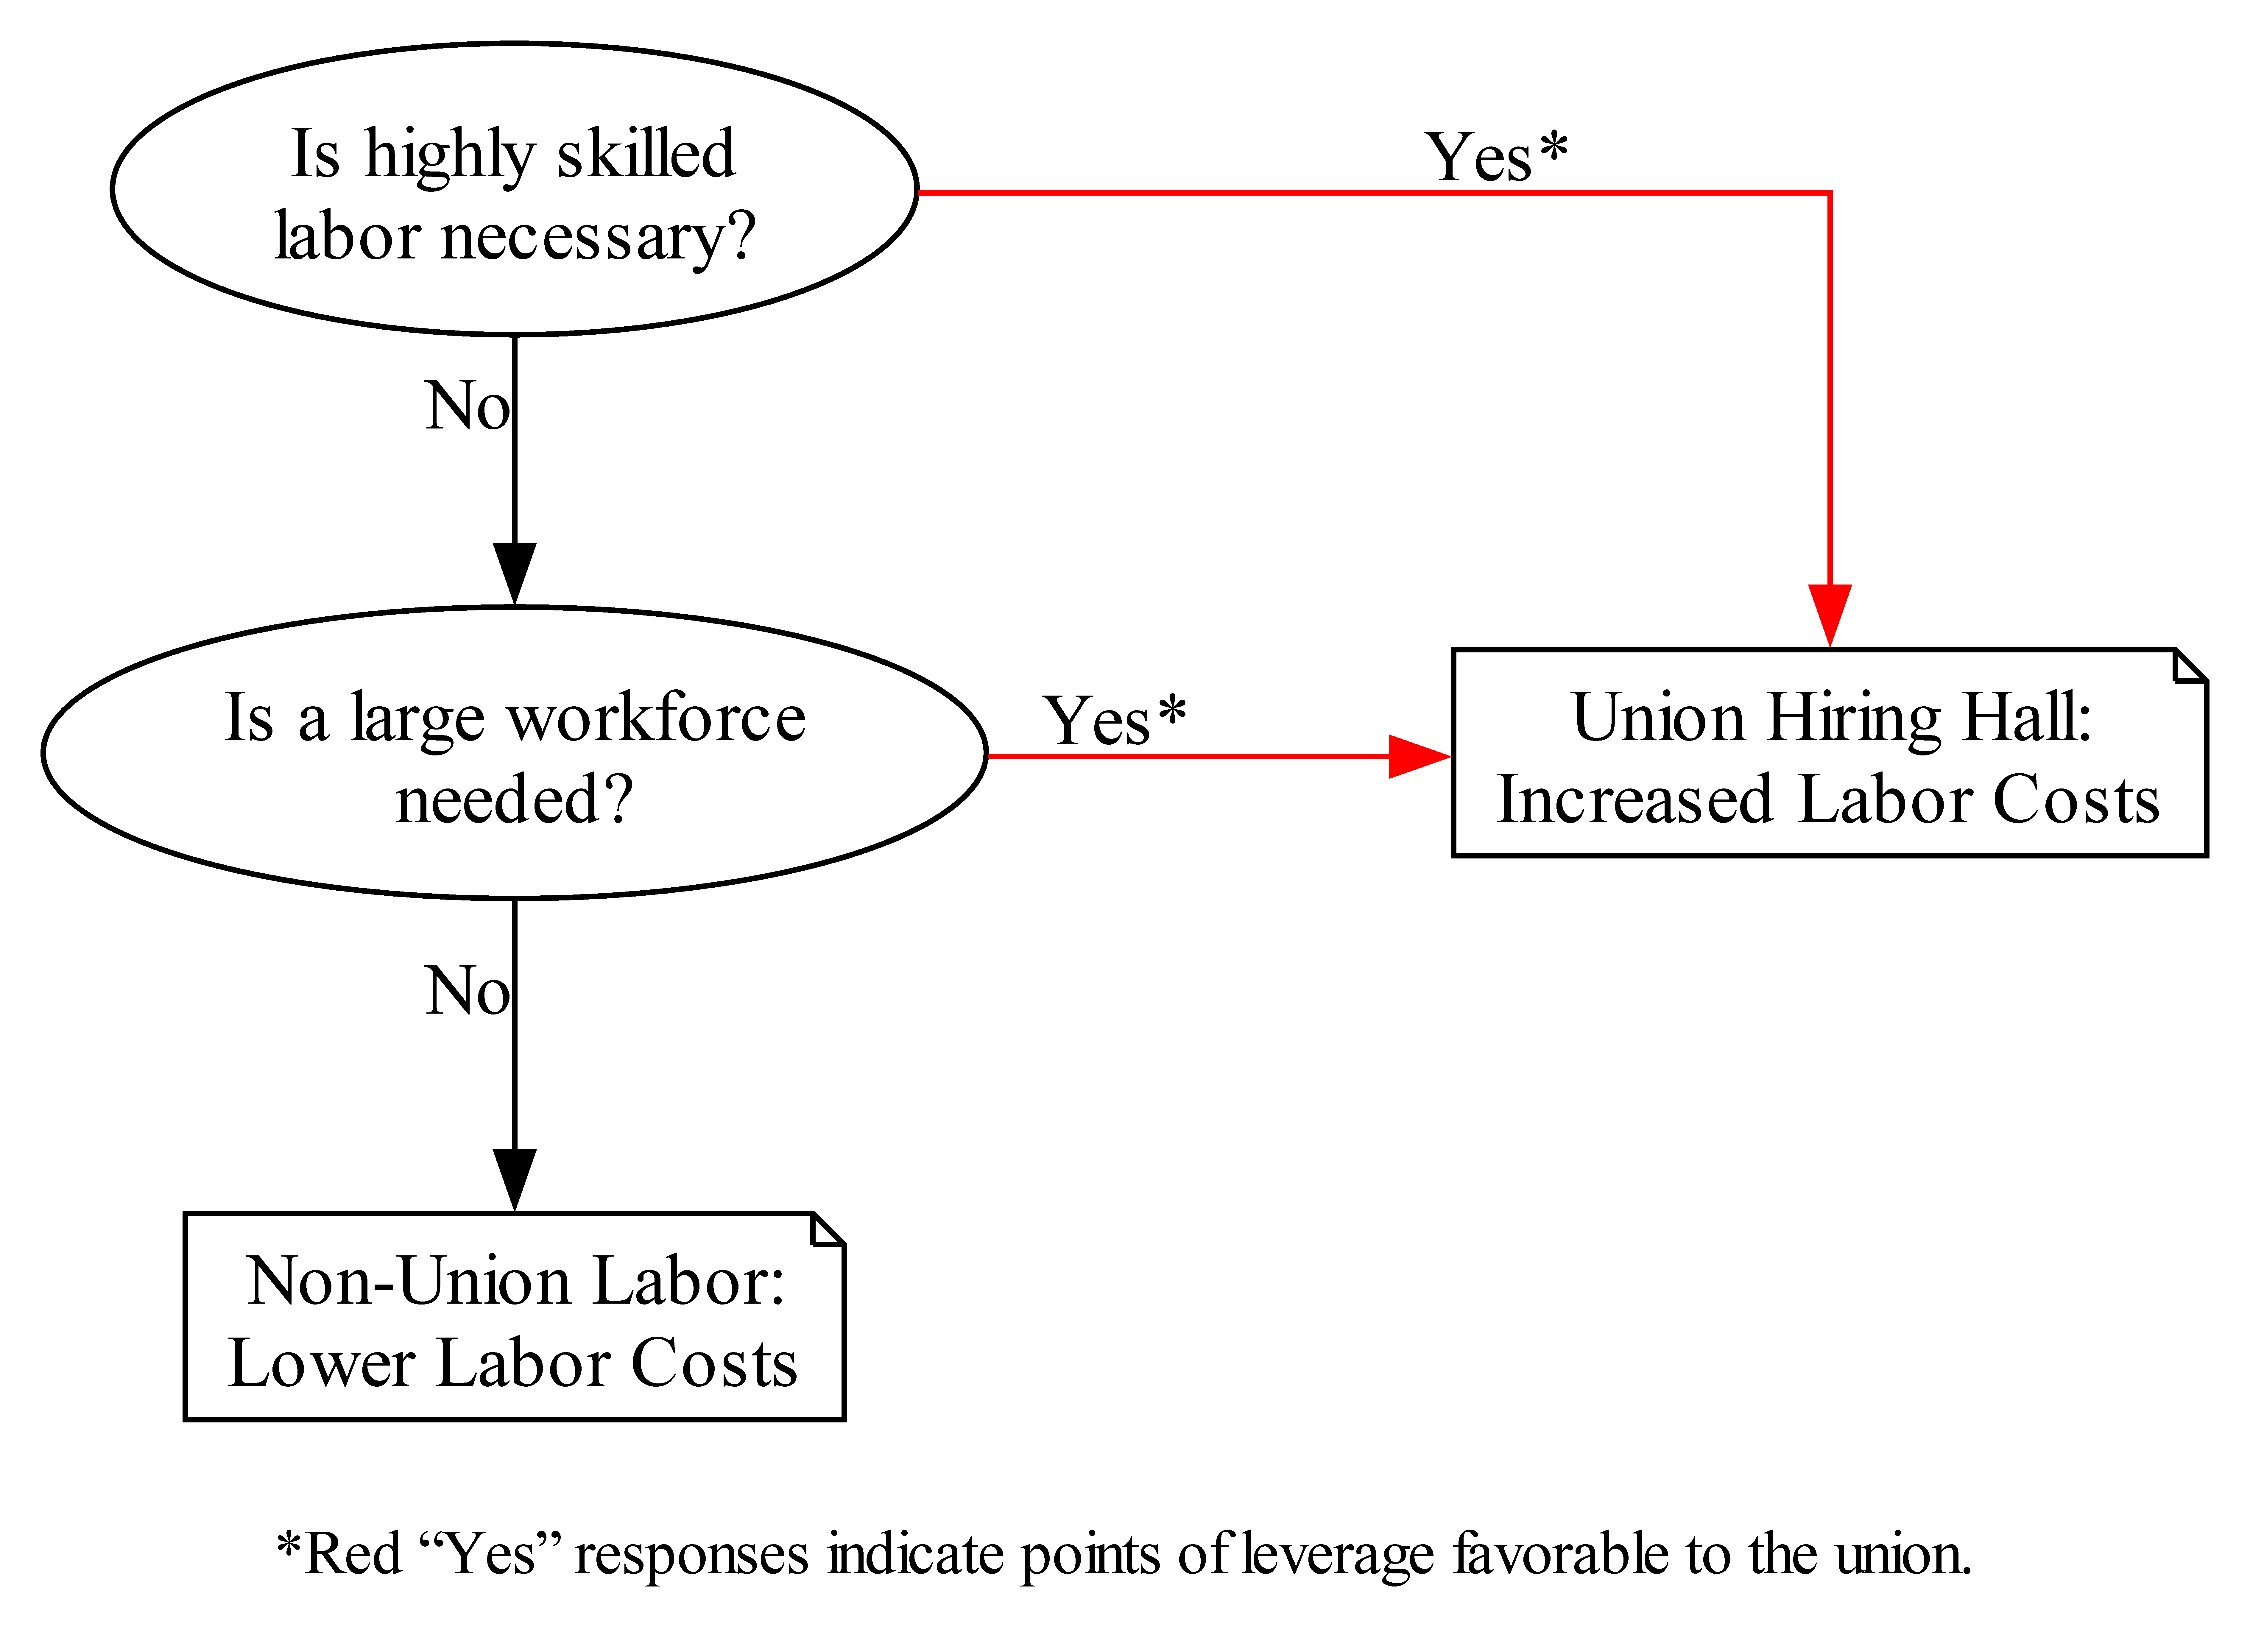
\includegraphics[width=0.8\textwidth]{images/union_power_red}
  \captionsetup{justification=centering, singlelinecheck=false, margin=2cm} 
  \caption{Since negotitations between construction unions and employers are voluntary, construction unions typically have more leverage where the employer requires a more skilled workforce or where the job is large and requires many employees.}
  \label{fig:union_power_red}
\end{figure}



\newpage

\begin{center}
{\bfseries Notes}
\end{center}

\noindent
.
\newpage
\begin{center}
{\bfseries Bibliography}
\end{center}

% \printbibliography

\end{document}
